\setlength{\tabcolsep}{3pt}
\begin{table*}[ht]
  \centering
  \begin{tabular}{crrrrrrrrrrrrrrr}
    & \multicolumn{3}{c}{xml} & \multicolumn{3}{c}{dna} & \multicolumn{3}{c}{psd7003} & \multicolumn{3}{c}{protein} & \multicolumn{3}{c}{comptree}\\
    &  \multicolumn{3}{c}{(23,551,472)} & \multicolumn{3}{c}{(32,747,474)} & \multicolumn{3}{c}{(42,611,636)} & \multicolumn{3}{c}{(60,160,372)} & \multicolumn{3}{c}{(2,147,483,646)}\\
\hline
    $p$ & \verb|psta| & \verb|libcds| & \verb|sdsl|  & \verb|psta| & \verb|libcds| & \verb|sdsl| & \verb|psta| & \verb|libcds| & \verb|sdsl| & \verb|psta| & \verb|libcds| & \verb|sdsl| & \verb|psta| & \verb|libcds| & \verb|sdsl|\\
\hline
 1   &  .99  &  9.95  & .60  &  1.01 & 10.68  & .64  &  1.04  & 10.73  & .63  &  .99   &  10.16  &  .61   & 1.00  & 11.59  & .69   \\
 2   &  1.96 &  19.71 & 1.19 &  1.98 & 21.01  & 1.27 &  2.06  & 21.33  & 1.26 &  1.98  &  20.26  &  1.22  & 1.98  & 22.93  & 1.36  \\
 4   &  3.77 &  38.00 & 2.30 &  3.88 & 41.18  & 2.48 &  3.94  & 40.84  & 2.41 &  3.92  &  39.99  &  2.41  & 3.82  & 44.33  & 2.62  \\
 6   &  5.25 &  52.84 & 3.20 &  5.43 & 57.73  & 3.48 &  5.63  & 58.30  & 3.44 &  5.46  &  55.77  &  3.36  & 5.50  & 63.82  & 3.78  \\
 8   &  7.14 &  71.89 & 4.36 &  7.30 & 77.58  & 4.67 &  6.89  & 71.36  & 4.21 &  7.49  &  76.45  &  4.60  & 7.64  & 88.64  & 5.25  \\
 10  &  8.09 &  81.46 & 4.94 &  8.42 & 89.43  & 5.39 &  6.72  & 69.66  & 4.11 &  7.14  &  72.97  &  4.39  & 9.14  & 106.01 & 6.28  \\
 12  &  7.58 &  76.38 & 4.63 &  7.83 & 83.19  & 5.01 &  7.97  & 82.59  & 4.87 &  9.56  &  97.62  &  5.88  & 10.54 & 122.26 & 7.24  \\
 14  &  8.28 &  83.36 & 5.05 &  8.39 & 89.18  & 5.37 &  8.74  & 90.63  & 5.34 &  9.36  &  95.64  &  5.76  & 11.94 & 138.47 & 8.20  \\
 16  &  7.08 &  71.34 & 4.32 &  8.41 & 89.39  & 5.38 &  7.52  & 77.90  & 4.59 &  8.48  &  86.57  &  5.21  & 14.20 & 164.75 & 9.75  \\
 18  &  7.23 &  72.77 & 4.41 &  5.76 & 61.23  & 3.69 &  10.19 & 105.59 & 6.22 &  9.36  &  95.61  &  5.76  & 14.91 & 172.99 & 10.24\\
 20  &  7.18 &  72.30 & 4.38 &  8.41 & 89.37  & 5.38 &  8.30  & 85.99  & 5.07 &  11.86 &  121.10 &  7.29  & 15.93 & 184.85 & 10.94\\
 22  &  7.43 &  74.84 & 4.53 &  7.69 & 81.72  & 4.92 &  7.98  & 82.75  & 4.88 &  7.83  &  79.99  &  4.82  & 17.20 & 199.60 & 11.82\\
 24  &  5.75 &  57.89 & 3.51 &  7.16 & 76.10  & 4.58 &  9.31  & 96.53  & 5.69 &  9.73  &  99.35  &  5.98  & 17.68 & 205.17 & 12.15\\
 26  &  6.74 &  67.88 & 4.11 &  8.82 & 93.69  & 5.64 &  9.18  & 95.09  & 5.60 &  11.00 &  112.38 &  6.77  & 18.58 & 215.54 & 12.76\\
 28  &  4.48 &  45.09 & 2.73 &  5.80 & 61.62  & 3.71 &  5.59  & 57.98  & 3.42 &  6.54  &  66.76  &  4.02  & 19.31 & 224.00 & 13.26\\
 30  &  4.91 &  49.49 & 3.00 &  9.81 & 104.26 & 6.2  &  6.25  & 64.81  & 3.82 &  8.95  &  91.41  &  5.50  & 19.17 & 222.38 & 13.17\\
 32  &  3.51 &  35.30 & 2.14 &  5.06 & 53.78  & 3.24 &  6.60  & 68.41  & 4.03 &  5.82  &  59.47  &  3.58  & 19.28 & 223.67 & 13.24\\
 \hline
\end{tabular}
\caption{Speedup.}
\label{tbl:speedup}
\end{table*}


In Table \ref{tbl:speedup} we report speedups for five different
inputs. Columns \verb+xml+, \verb+dna+, \verb+protein+ correspond to
LZ78 parsings of the DNA, protein and XML texts from the Pizza \&
Chili corpus\footnote{\url{http://pizzachili.dcc.uchile.cl}}, column
\verb+psd7003+ correspond to the XMLData Repository from University of
Washington\footnote{\url{http://www.cs.washington.edu/research/xmldatasets/}}
and column \verb+comptree+ is a complete binary tree of depth
30. Below of each corpus' name we report its size, the number of
parentheses of their folklore encoding (i.e., the number of ``real''
nodes is that figure divided by 2). For each corpus, we report three
values: \verb+psta+ which is the speedup of the sequential version of
our parallel algorithm (i.e., without the parallel extensions) over
our parallel algorithm; \verb+libcds+, the speedup of the
\verb+libcds+ library over our parallel algorithm and \verb+sdsl+ the
speedup of sdsl library over our parallel algorithm. Column \verb+p+
shows the number of threads that were tested (threads are 1:1 to the
number of physical cores). We repeated each experiment three times and
recorded the minimum time, assuming that slightly larger values of any
given experiment are just ``noise'' from external processes such as
operating system and networking tasks\footnote{For experiments with
  more corpus, please visit
  \url{http://www.inf.udec.cl/~josefuentes/spaa2015}}.

\begin{figure}[ht]
  \centering
  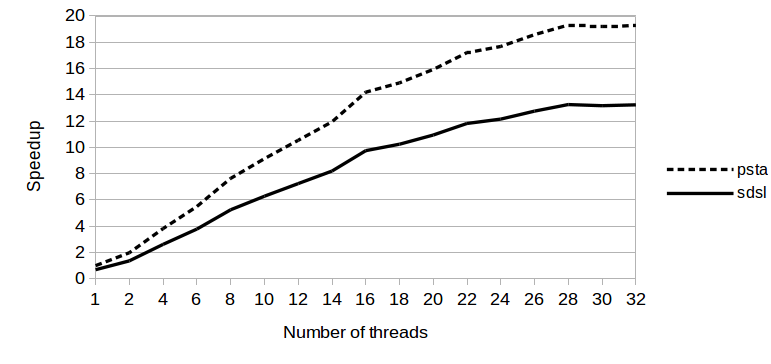
\includegraphics[scale=0.3]{./images/Speedup.png}
  \caption{Speedup of comptree corpus}
  \label{fig:speedup} 
\end{figure}

We do not optimize our code, we just care to generate a correct
implementation, that is why our sequential version is slower than
state-of-the-art sequential implementations such as
\verb+sdsl+. However, our implementation does have a similar behavior
compared to those state-of-the-art implementations. To make the
results more intuitive, Figure \ref{fig:speedup} shows the speedup of
the largest corpus. The \verb+libcds+ library is not shown in Figure
\ref{fig:speedup} because the times we obtained were not comparable to
either ours or \verb+sdsl+. They were slower by an order of
magnitude. When the number of threads is a power of two: 1, 2, 4, 8,
16, the speedup of \verb+psta+ is almost linear. This happens because
when the number of threads is a power of two, our algorithm can assign
exactly one subtree per thread (see Algorithm \ref{algo:PSTA2}),
distributing the work homogeneously (without enrolling the
work-stealing scheduler). When the number of threads is not a power of
two, some threads have to process more than one subtree and other
threads just process one, degrading the performance. Even though this
strategy degrades the performance a little, the threads are always
working, which is a good feature on parallel processing. Since the
machine where we run our experiments has 32 physical cores and other
processes were running, such as, the operating system, the speedup
near the 32nd thread does not reach a linear behavior\footnote{We
  could not test the ``breakeven'' characteristic of our algorithm
  because we do not have a machine with enough physical cores.}. 


Since {\tt psta} generates tasks that work on different memory
regions, the generated cache misses \Leo{false sharing is misses} do
not degrade the performance. The same effect is present on
\emph{Domain Decomposition Algorithms}. Although the decomposition of
the {\tt RMMT} was not evident, we could produce a decomposition that
generated a competitive algorithm.
	
\begin{table}[ht]
  \centering
  \begin{tabular}{crrrrr}
\hline
    & xml & dna & psd7003 & protein & comptree\\
\hline
 \verb|psta|   &  1.46  &  1.74  & 2.78  &  3.30 & 112.01\\
 \verb|libcds|   &  .42 &  .58 & .77 &  1.08 & 38.25\\
 \verb|sdsl|   &  .95 &  1.31 & 1.73 &  2.41 & 76.40\\
 \hline
\end{tabular}
\caption{Peak of memory consumption. Values are in MB}
\label{tbl:memory_consumption}
\end{table}

Table \ref{tbl:memory_consumption} shows memory consumption for the
same corpora in Table \ref{tbl:speedup}. To measure memory , we
monitored how much memory was allocated with \emph{malloc} and
released with \emph{free} at execution time, recording the peak of
consumption. We only consider memory allocated during construction,
but not memory allocated to store the parentheses sequence. We only
report memory consumption of {\tt psta} with $p=1$, because the
consumption associated to thread scheduling was negligible. Even
though {\tt psta} consumes more memory than the baseline algorithms,
it is still a constant factor with respect to the other two
implementations. The use of the memory allocated to arrays
$e^{\prime}$, $m^{\prime}$, $M^{\prime}$ and $n^{\prime}$ to save the
partial excess values was an important feature of our algorithm, since
{\tt psta} could use the same amount of memory than its sequential
version. In other words, memory consumption does not grow as a
function of $p$.

In the experiments, {\tt psta} uses more memory than the baselines
because we assume 16 bits per excess value. If we use a simplification
of Algorithm \ref{algo:PSTA1} to calculate the depth $d$ of the input
sequence (the maximum excess value), we could use it to allocate just
$\lg (d)$ bits per excess value, saving memory and improving
performance, and thus reducing memory transfers.














